\subsection{Deep Deterministick Policy Gradienten (DDPG)}

Während das Deep Q-Network (DQN) für jeden Zustand s eine Bewertung aller möglichen Aktionen a liefert, wie in Abbildung \ref{fig:dqn} illustriert, stößt es in kontinuierlichen Aktionsräumen an seine Grenzen. Die Unzulänglichkeit von DQN in solchen Szenarien -- da die Bewertung einer unendlichen Anzahl von Aktionen nicht praktikabel ist -- führt uns zu fortgeschritteneren Methoden wie dem Deep Deterministic Policy Gradient (DDPG).\cite{morales2020grokking}).

\paragraph{Einführung in die Actor-Critic-Architektur des DDPG}

Der DDPG-Algorithmus repräsentiert einen bedeutenden Fortschritt im Reinforcement Learning für kontinuierliche Aktionsräume. Zentral für seine Funktionsweise ist die Actor-Critic-Architektur, die aus zwei Schlüsselkomponenten besteht: dem Actor und dem Critic, die beide durch tiefe neuronale Netze approximiert werden \cite{SuttonBarto2018}.


\begin{figure}[htbp]
\centering
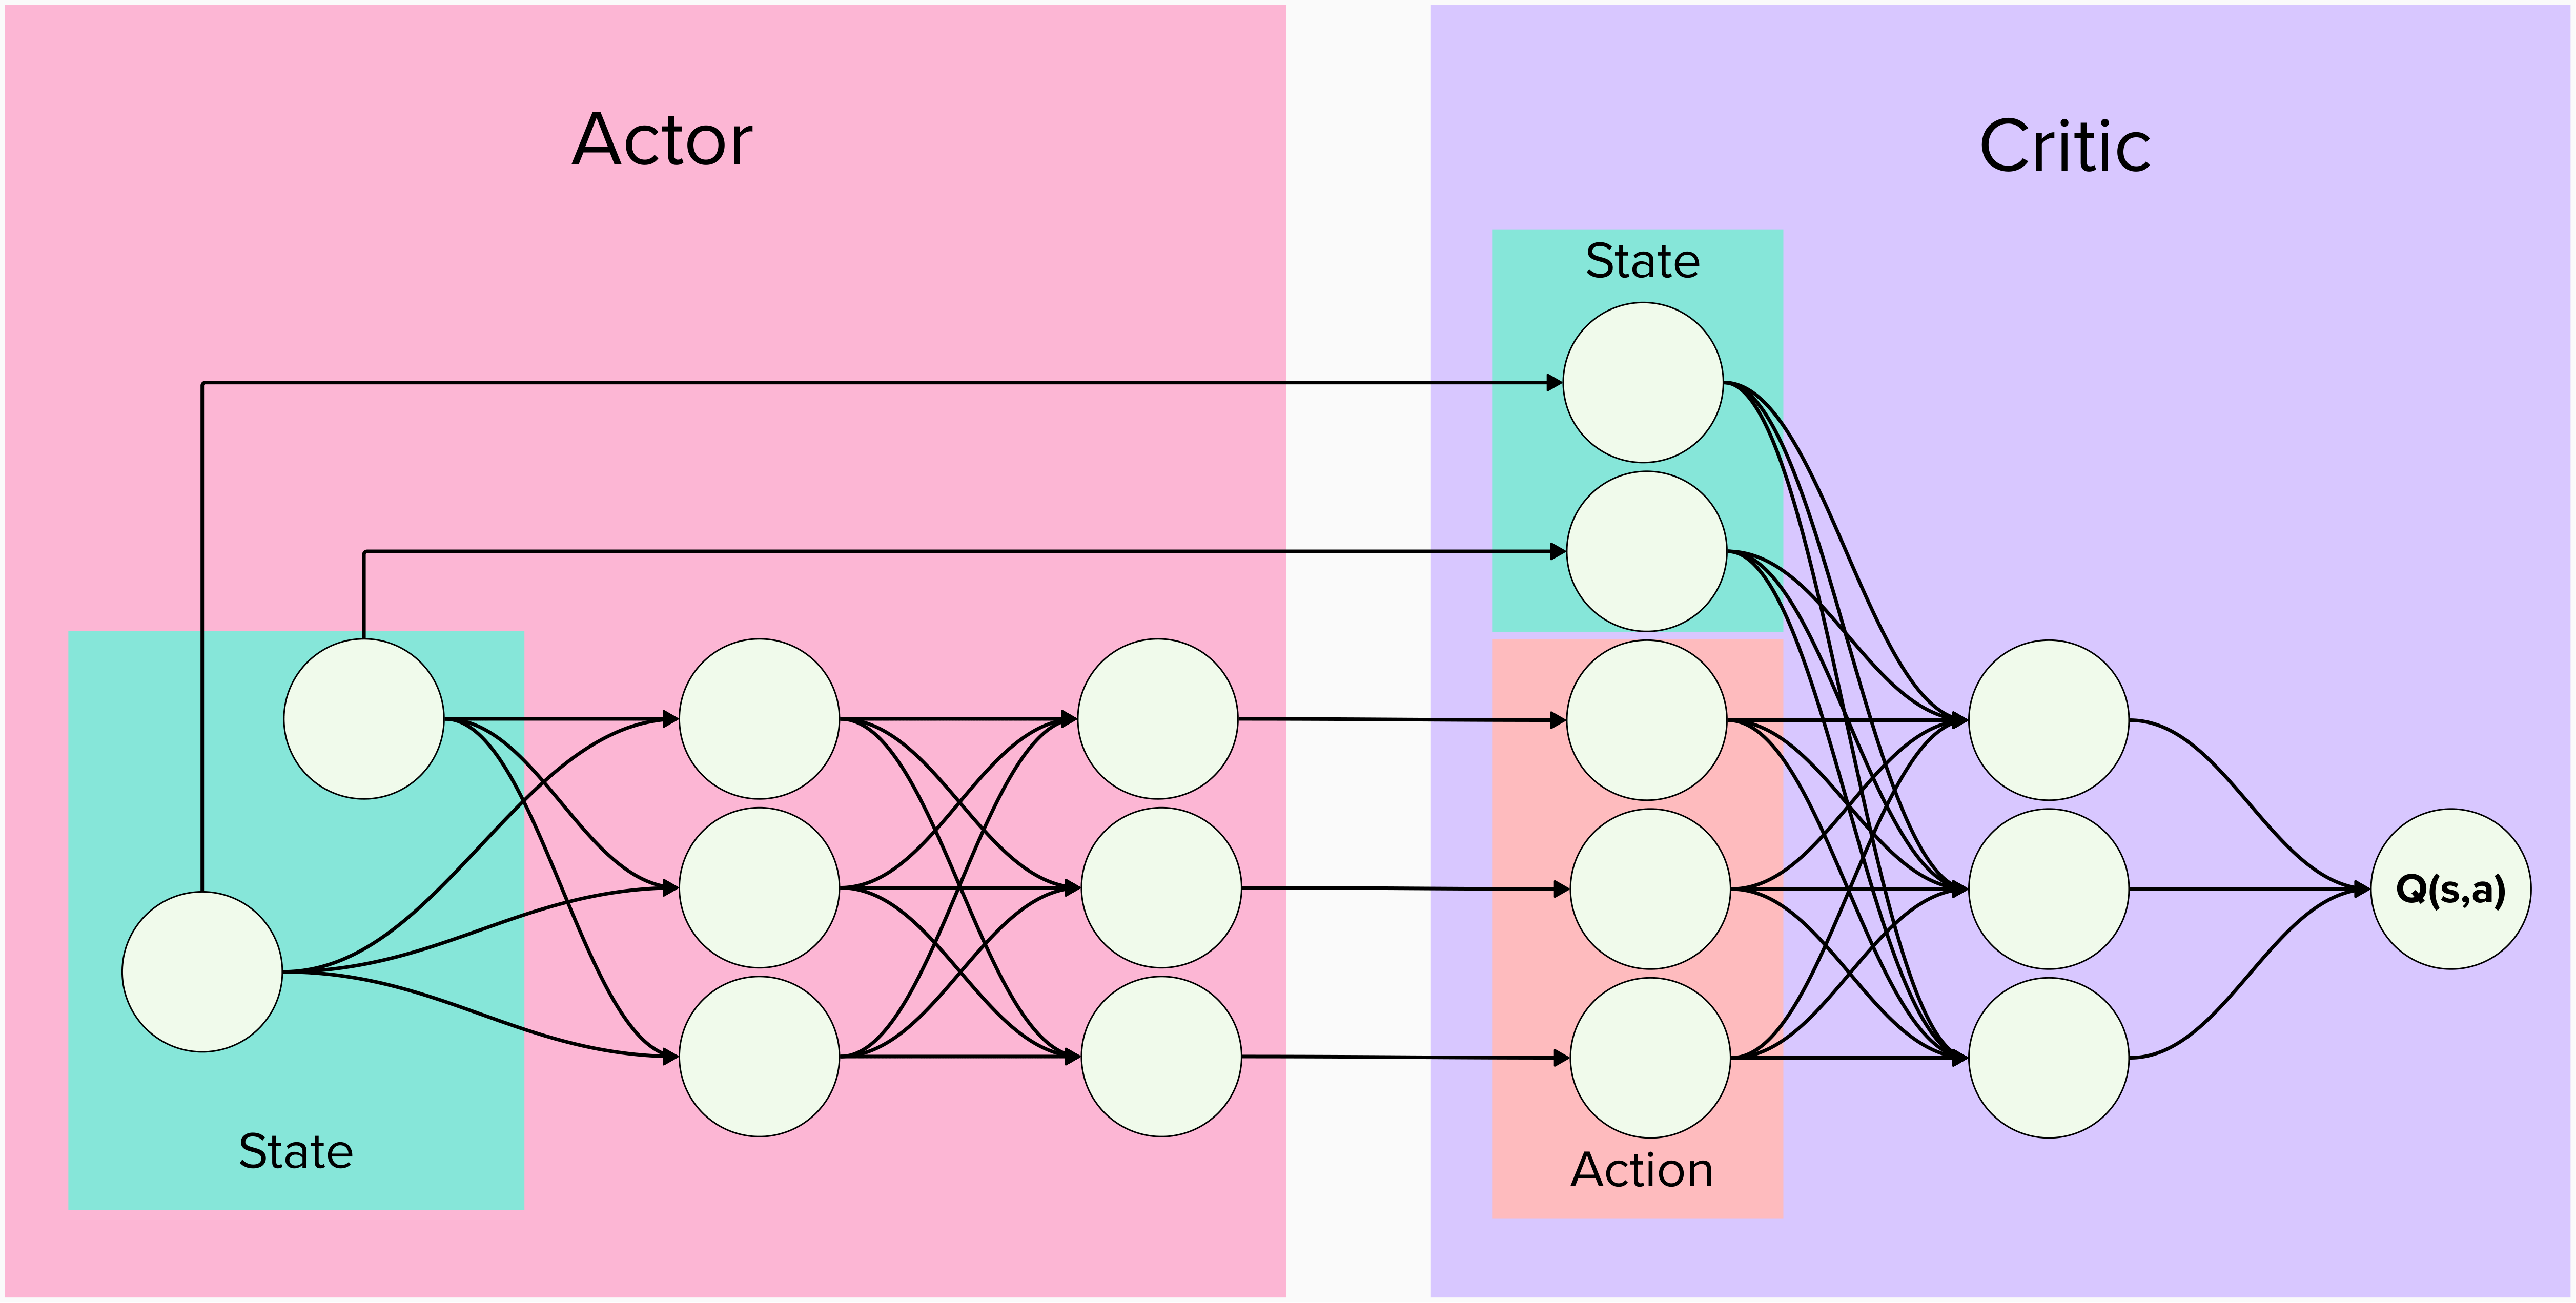
\includegraphics[width=0.65\textwidth]{2Grundlagen/35Actor_Critick.png}
\caption{Illustration des Actors und Critics im DDPG-Algorithmus.}
\label{fig:actor_critick}
\end{figure}

\paragraph{Die Rolle des Actors}
Der Actor \ref{fig:actor_critick} hat die Aufgabe, eine optimale Policy \(\mu(s)\) zu erlernen, die für jeden gegebenen Zustand \(s\) eine Aktion \(a\) ausgibt, mit dem Ziel, den erwarteten Reward zu maximieren \cite{SuttonBarto2018}. Diese Policy-Funktion wird in einem kontinuierlichen Aktionsraum direkt modelliert, wobei jede Aktion ein kontinuierlicher Wert ist. Der Actor ist daher das Entscheidungselement innerhalb der Architektur \cite{SuttonBarto2018}.


\paragraph{Die Funktion des Critics}
\label{sec: Rolle des Critics}
Der Critic \ref{fig:actor_critick} hingegen bewertet die Aktionen, die vom Actor vorgeschlagen werden wie in Abbildung \ref{fig:get_q_value_critic} gezeigt. Er nimmt den aktuellen Zustand und die vom Actor vorgeschlagene Aktion auf und schätzt den Q-Wert \( Q(s,a) \). Diese Schätzung repräsentiert den erwarteten zukünftigen Reward, der aus der Ausführung der Aktion \( a \) im Zustand \( s \) resultiert, noch bevor die eigentliche Simulation in der Umgebung gestartet wird \cite{SuttonBarto2018}. Somit versucht der Critic, die Qualität einer Aktion im Kontext des aktuellen Zustands zu bewerten und liefert dem Actor Feedback, das zur Optimierung der Policy verwendet wird.

\paragraph{Die Actor-Critic-Interaktion}
In Abbildung \ref{fig:actor_critick} ist die Interaktion zwischen dem Actor und dem Critic illustriert. Der Actor generiert Aktionen basierend auf der aktuellen Policy, und der Critic bewertet diese Aktionen, indem er den Q-Wert zur Verfügung stellt. Diese Interaktion ermöglicht es dem DDPG-Algorithmus, sowohl die optimale Policy als auch die Wertfunktion effektiv zu lernen \cite{SuttonBarto2018}.


\paragraph{Aktualisierung des Critics im DDPG}

Die Aktualisierung des Critics im Deep Deterministic Policy Gradient Algorithmus ist ein entscheidender Schritt für das effektive Lernen von handlungsorientierten Strategien in kontinuierlichen Aktionsräumen. Die grundlegende Idee des DDPG ist es, die Stärken von Q-Learning \ref{eq: update q learning} und Policy Gradient Methoden \ref{eq:policy_gradient} zu kombinieren, um die Effizienz des Lernprozesses in solchen Umgebungen zu verbessern \cite{Lillicrap2016DDPG}.


\paragraph{Update-Prinzip des Critics}
\begin{figure}[htbp]
\centering
  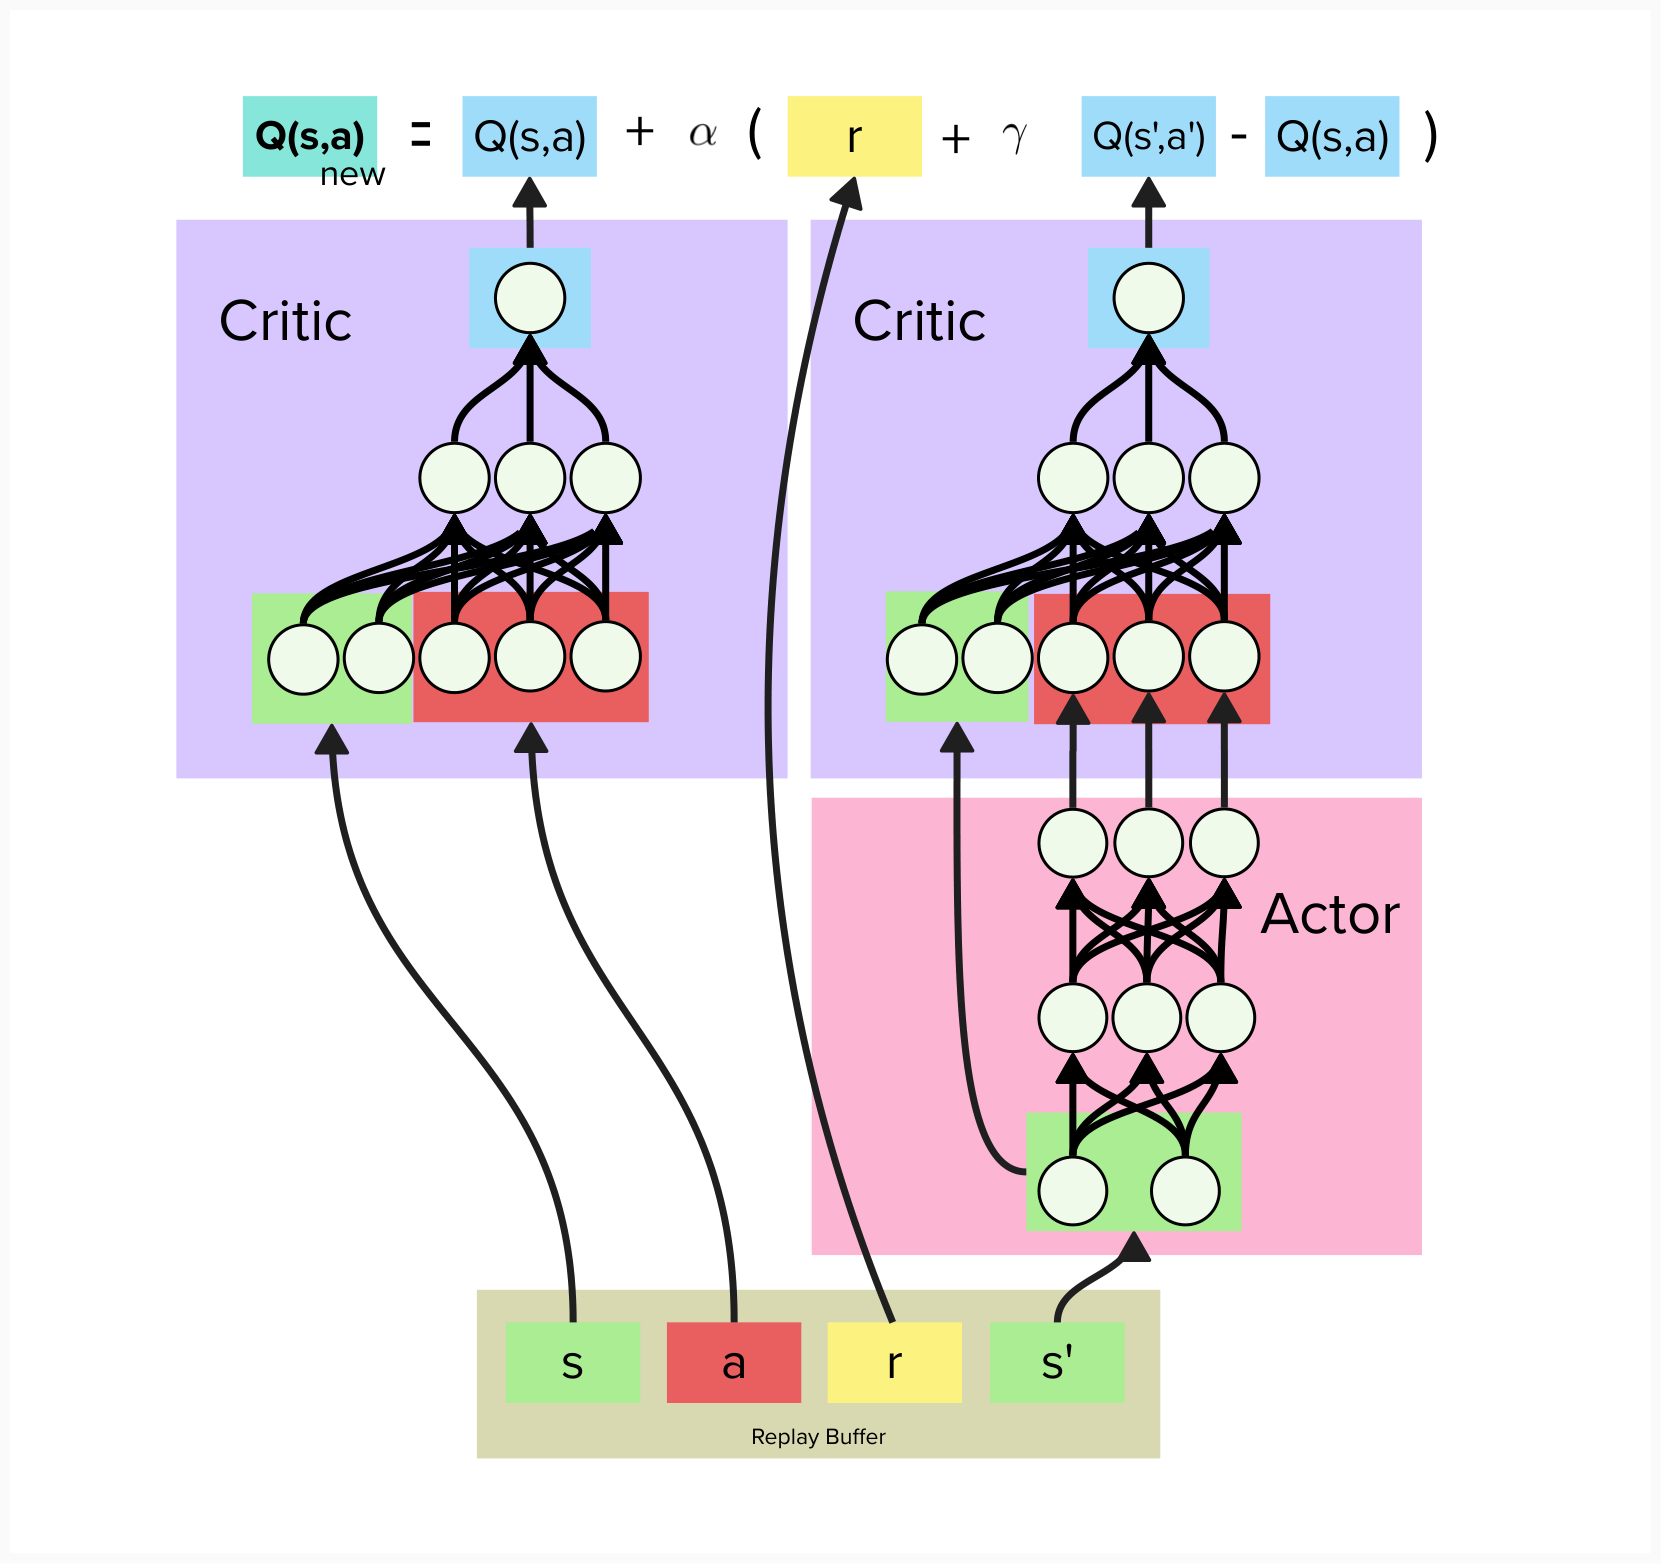
\includegraphics[width=0.70\textwidth, trim=10px 10px 10px 10px, clip]{2Grundlagen/35Q_value_Critick.png}
  \captionof{figure}[Berechnung des Q-Werts]{Berechnung des Q-Werts durch den Critic (Quelle: \cite{wei2020ddpg}).}
  \label{fig:get_q_value_critic}
\end{figure}
Der Critic bewertet die Politik des Actors, indem er die Q-Werte für die vom Actor vorgeschlagenen Aktionen schätzt. Diese Q-Werte repräsentieren das erwartete zukünftige Reward für den Zustand-Aktions-Paar (\(s, a\)). Der Critic wird aktualisiert, indem der Temporal Difference (TD) Error minimiert wird \ref{eq:Ketten Regel},  der die Differenz zwischen den geschätzten Q-Werten und den tatsächlichen Rewards aus der Umgebung widerspiegelt \cite{Wu2018AggregatedMultiDDPG}. Die Update-Regel für den Critic ist eine Variante der Bellman-Gleichung \ref{eq: Bellman } , die im DQN verwendet wird \ref{eq: update q learning}, und kann formal durch die folgende Gleichung ausgedrückt werden:



\begin{equation}
		Q(s,a) \leftarrow Q(s,a) + \alpha \cdot (r + \gamma \cdot Q(s',\mu(s') - Q(s,a)))
		\label{eq:critick update}
\end{equation}

Hierbei ist \( \alpha \) die Lernrate, \( r \) der sofortige Reward, \( \gamma \) der Diskontierungsfaktor für zukünftige Rewards, und \( \mu(s') \) die Policy des Actors, die den nächsten Zustand \( s' \) auf die nächste Aktion abbildet, wie in Abbildung \ref{fig:get_q_value_critic} gezeigt.



Der TD Error für das Training des Critics kann dann als die Differenz zwischen dem geschätzten Q-Wert und dem Target-Q-Wert definiert werden:
\[ TD_{error} = Q_{target}(s_t, a_t) - Q(s_t, a_t) \]
Diese Diskrepanz wird quadriert \ref{eq:cost_function}, um als Loss-Funktion zu fungieren, die dann minimiert wird , um das Lernen zu verbessern \ref{eq:partial_derivative} \cite{SuttonBarto2018}.

\begin{figure}[htbp]
\centering
  \centering
  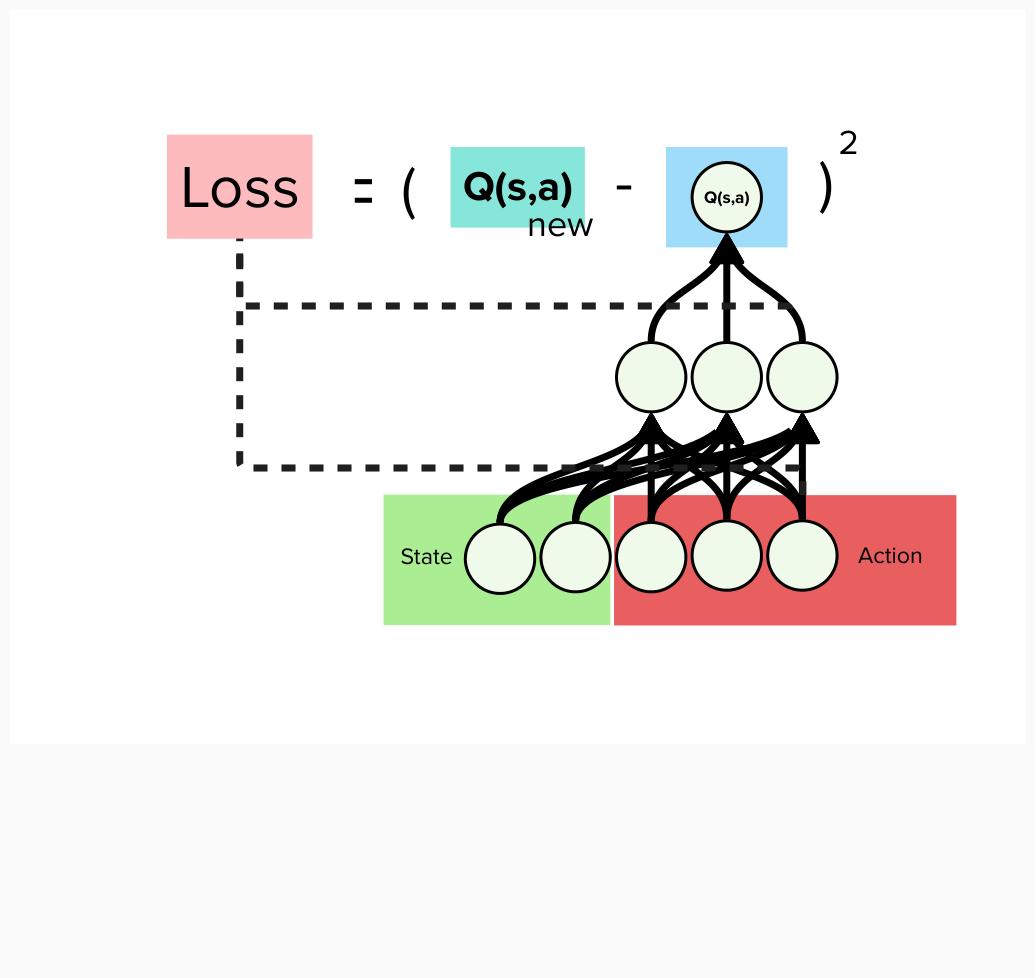
\includegraphics[width=0.45\textwidth, trim=10px 10px 10px 10px, clip]{2Grundlagen/35Q_value_Critick_update.png}
  \captionof{figure}[Aktualisierung des Q-Werts]{Aktualisierung des Q-Werts im Critic-Netzwerk.}
  \label{fig:update_q_value}
\end{figure}



\paragraph{Gradient Descent und Kettenregel}
Um die Gewichte des Critics zu aktualisieren, wird der Gradient Descent angewendet, wobei der Gradient der Loss-Funktion in Bezug auf die Gewichte berechnet \ref{eq: gradient matrix} und die Gewichte entsprechend angepasst werden \cite{aggarwal_neural_networks_2018}.




\paragraph{Bedeutung der Kritik}
Die Funktion des Critics ist es nicht nur, die Aktionen des Actors zu bewerten, sondern auch, eine Lernsignal für den Actor zu generieren. Dies geschieht durch die Rückkopplung des TD Errors an den Actor, wodurch dieser informiert wird, welche Aktionen zu einer Verbesserung oder Verschlechterung des erwarteten Rewards führen. Der Actor nutzt diese Information, um seine Policy in Richtung von Aktionen zu steuern, die zu einem höheren Reward führen \cite{Luck2019ImprovedExploration}.


\paragraph{Optimierung des Actor-Netzwerks im DDPG}

In Anlehnung an die zuvor dargestellte Aktualisierung des Critics ist das Ziel des Actor-Updates, eine Policy-Funktion zu erlernen, die Aktionen ausgibt, um den erwarteten Reward zu maximieren. Dieser Lernprozess basiert auf der Rückkopplung durch den Critic, der bereits präzise Q-Werte liefert. Die Aktualisierung erfolgt durch Anwendung eines Gradienten-Ascent-Verfahrens, welches auf die Maximierung der Q-Werte ausgerichtet ist \cite{Lillicrap2016DDPG, Wu2018AggregatedMultiDDPG}.


Die mathematische Darstellung des Updates wird durch die Gleichung ausgedrückt, die die Ableitung des Losses in Bezug auf die Parameter \(\theta_\mu\) des Actor-Netzwerks darstellt:
\begin{equation}
\nabla_{\theta_\mu} \text{LOSS}_{Actor} = -\mathbb{E}_{s \sim \mathcal{D}} \left[ \nabla_a Q(s, a)|_{a=\mu(s)} \nabla_{\theta_\mu} \mu(s) \right]
		\label{eq:actor update}
\end{equation}


\begin{figure}[htbp]
\centering
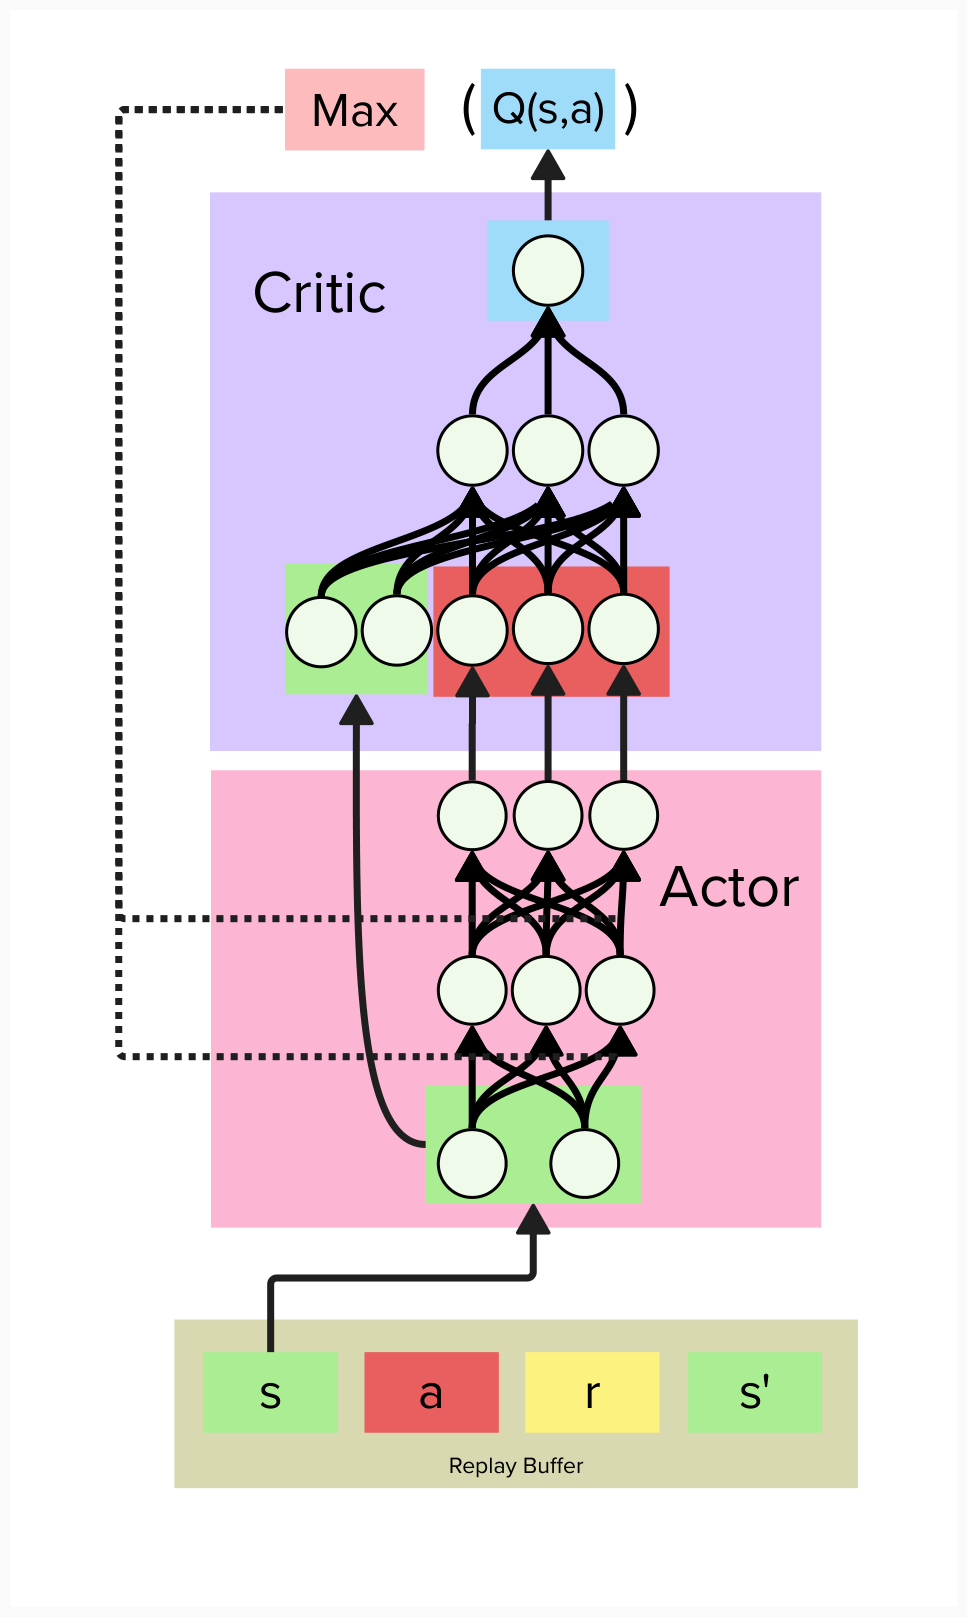
\includegraphics[width=0.45\textwidth, trim=10px 10px 10px 10px, clip]{2Grundlagen/35_update_actor.png}
\captionof{figure}[Aktualisierung des Actors]{Gradienten-Ascent für die Aktualisierung des Actors, um die Q-Werte zu maximieren. Der Actor nutzt die vom Critic berechneten Q-Werte, um die Policy-Funktion zu optimieren und den erwarteten Reward zu maximieren.}
\label{fig:update_actor}
\end{figure}

\paragraph{Der Update-Mechanismus des Actors}
Wie in Abbildung \ref{fig:update_actor} dargestellt, zielt das Update des Actors darauf ab, eine Policy-Funktion zu erlernen, die Aktionen so ausgibt, dass der erwartete Reward maximiert wird.Der Actor wählt Aktionen anhand der aktuellen Policy aus, die anschließend in der Umgebung ausgeführt werden, was zur Transition von Zustand \(s\) zu Zustand \(s'\) und zur Vergabe eines Rewards führt. Wie in \cite{Lillicrap2016DDPG} beschrieben, wird der Actor durch die Anwendung der Kettenregel \ref{eq:Ketten Regel} auf den erwarteten Return aus der Startverteilung aktualisiert, was eine direkte Anpassung der Actor-Parameter ermöglicht. Die Verlustfunktion des Actors wird durch die negativen Gradienten der Q-Werte in Bezug auf die Aktionen, berechnet an der Stelle der durch die Policy vorgeschlagenen Aktionen, definiert. Diese wird dann genutzt, um die Parameter der Actor-Policy in Richtung eines höheren erwarteten Rewards zu verschieben \cite{Lillicrap2016DDPG}.


\paragraph{Die Bedeutung der Aktualisierung des Actors}
Die Aktualisierung des Actors ist ein kritischer Schritt im Lernprozess, da sie das Trainingssignal für den Actor aus den Bewertungen des Critics ableitet. Diese Interaktion ermöglicht es dem Actor, seine Policy zu verbessern und optimale Aktionen im Kontext der gegebenen Umgebung auszuwählen \cite{Luck2019ImprovedExploration}. Die kontinuierliche Verbesserung der Policy durch den Actor führt zu einer verbesserten Entscheidungsfindung und letztlich zu einem höheren kumulativen Reward.

DDPG nutzt die Experience Replay-Technik, die zuerst in DQN eingeführt wurde \ref{eq:replay buffer}, um die Korrelation zwischen aufeinanderfolgenden Lernschritten zu reduzieren. Dies erhöht die Datenvarianz und hilft, eine stabilere und effektivere Lernumgebung zu schaffen, wie in \cite{Wu2018AggregatedMultiDDPG} beschrieben. 


\paragraph{Exploration und Exploitation im DDPG}

Der DDPG-Algorithmus erweitert die traditionelle \(\epsilon\)-greedy Strategie \ref{eq:epsilon_greedy} um eine raffinierte Explorationstaktik, bei der ein kontrolliertes Rauschen auf die Auswahl kontinuierlicher Aktionen angewendet wird. Dieses adaptive Rauschen, wie  Simulated-Annealing-Prozess \ref{sec:Simulated Annealing}, wird schrittweise verringert und ermöglicht so eine effektive Exploration des Aktionsraums. Durch diese graduelle Reduktion, verringert der Algorithmus die anfängliche Abhängigkeit von der Rauschintensität und fördert die Entdeckung optimaler Handlungsstrategien.


\paragraph{Integration von Experience Replay}

Neben dieser adaptiven Explorationsmethode implementiert DDPG auch die Erfahrungswiedergabe (siehe Gleichung \ref{eq:replay buffer}), ein Ansatz, der zuerst in DQN zum Einsatz kam. Diese Technik ist entscheidend, um die Abhängigkeiten zwischen aufeinanderfolgenden Stichproben zu beseitigen und sie als unabhängig und identisch verteilt zu behandeln, was die Stabilität des Lernprozesses deutlich erhöht \cite{Wu2018AggregatedMultiDDPG}. Die Anpassung des Actor-Netzwerks, das die zugrundeliegende Policy repräsentiert, folgt konsequent den Prinzipien der Kettenregel und der Rückpropagation, um eine konvergente Annäherung an die optimale Policy zu gewährleisten, die wiederum die Gesamteffizienz des Algorithmus steigert \cite{Wu2018AggregatedMultiDDPG}.

\begin{figure}[htbp]
\centering
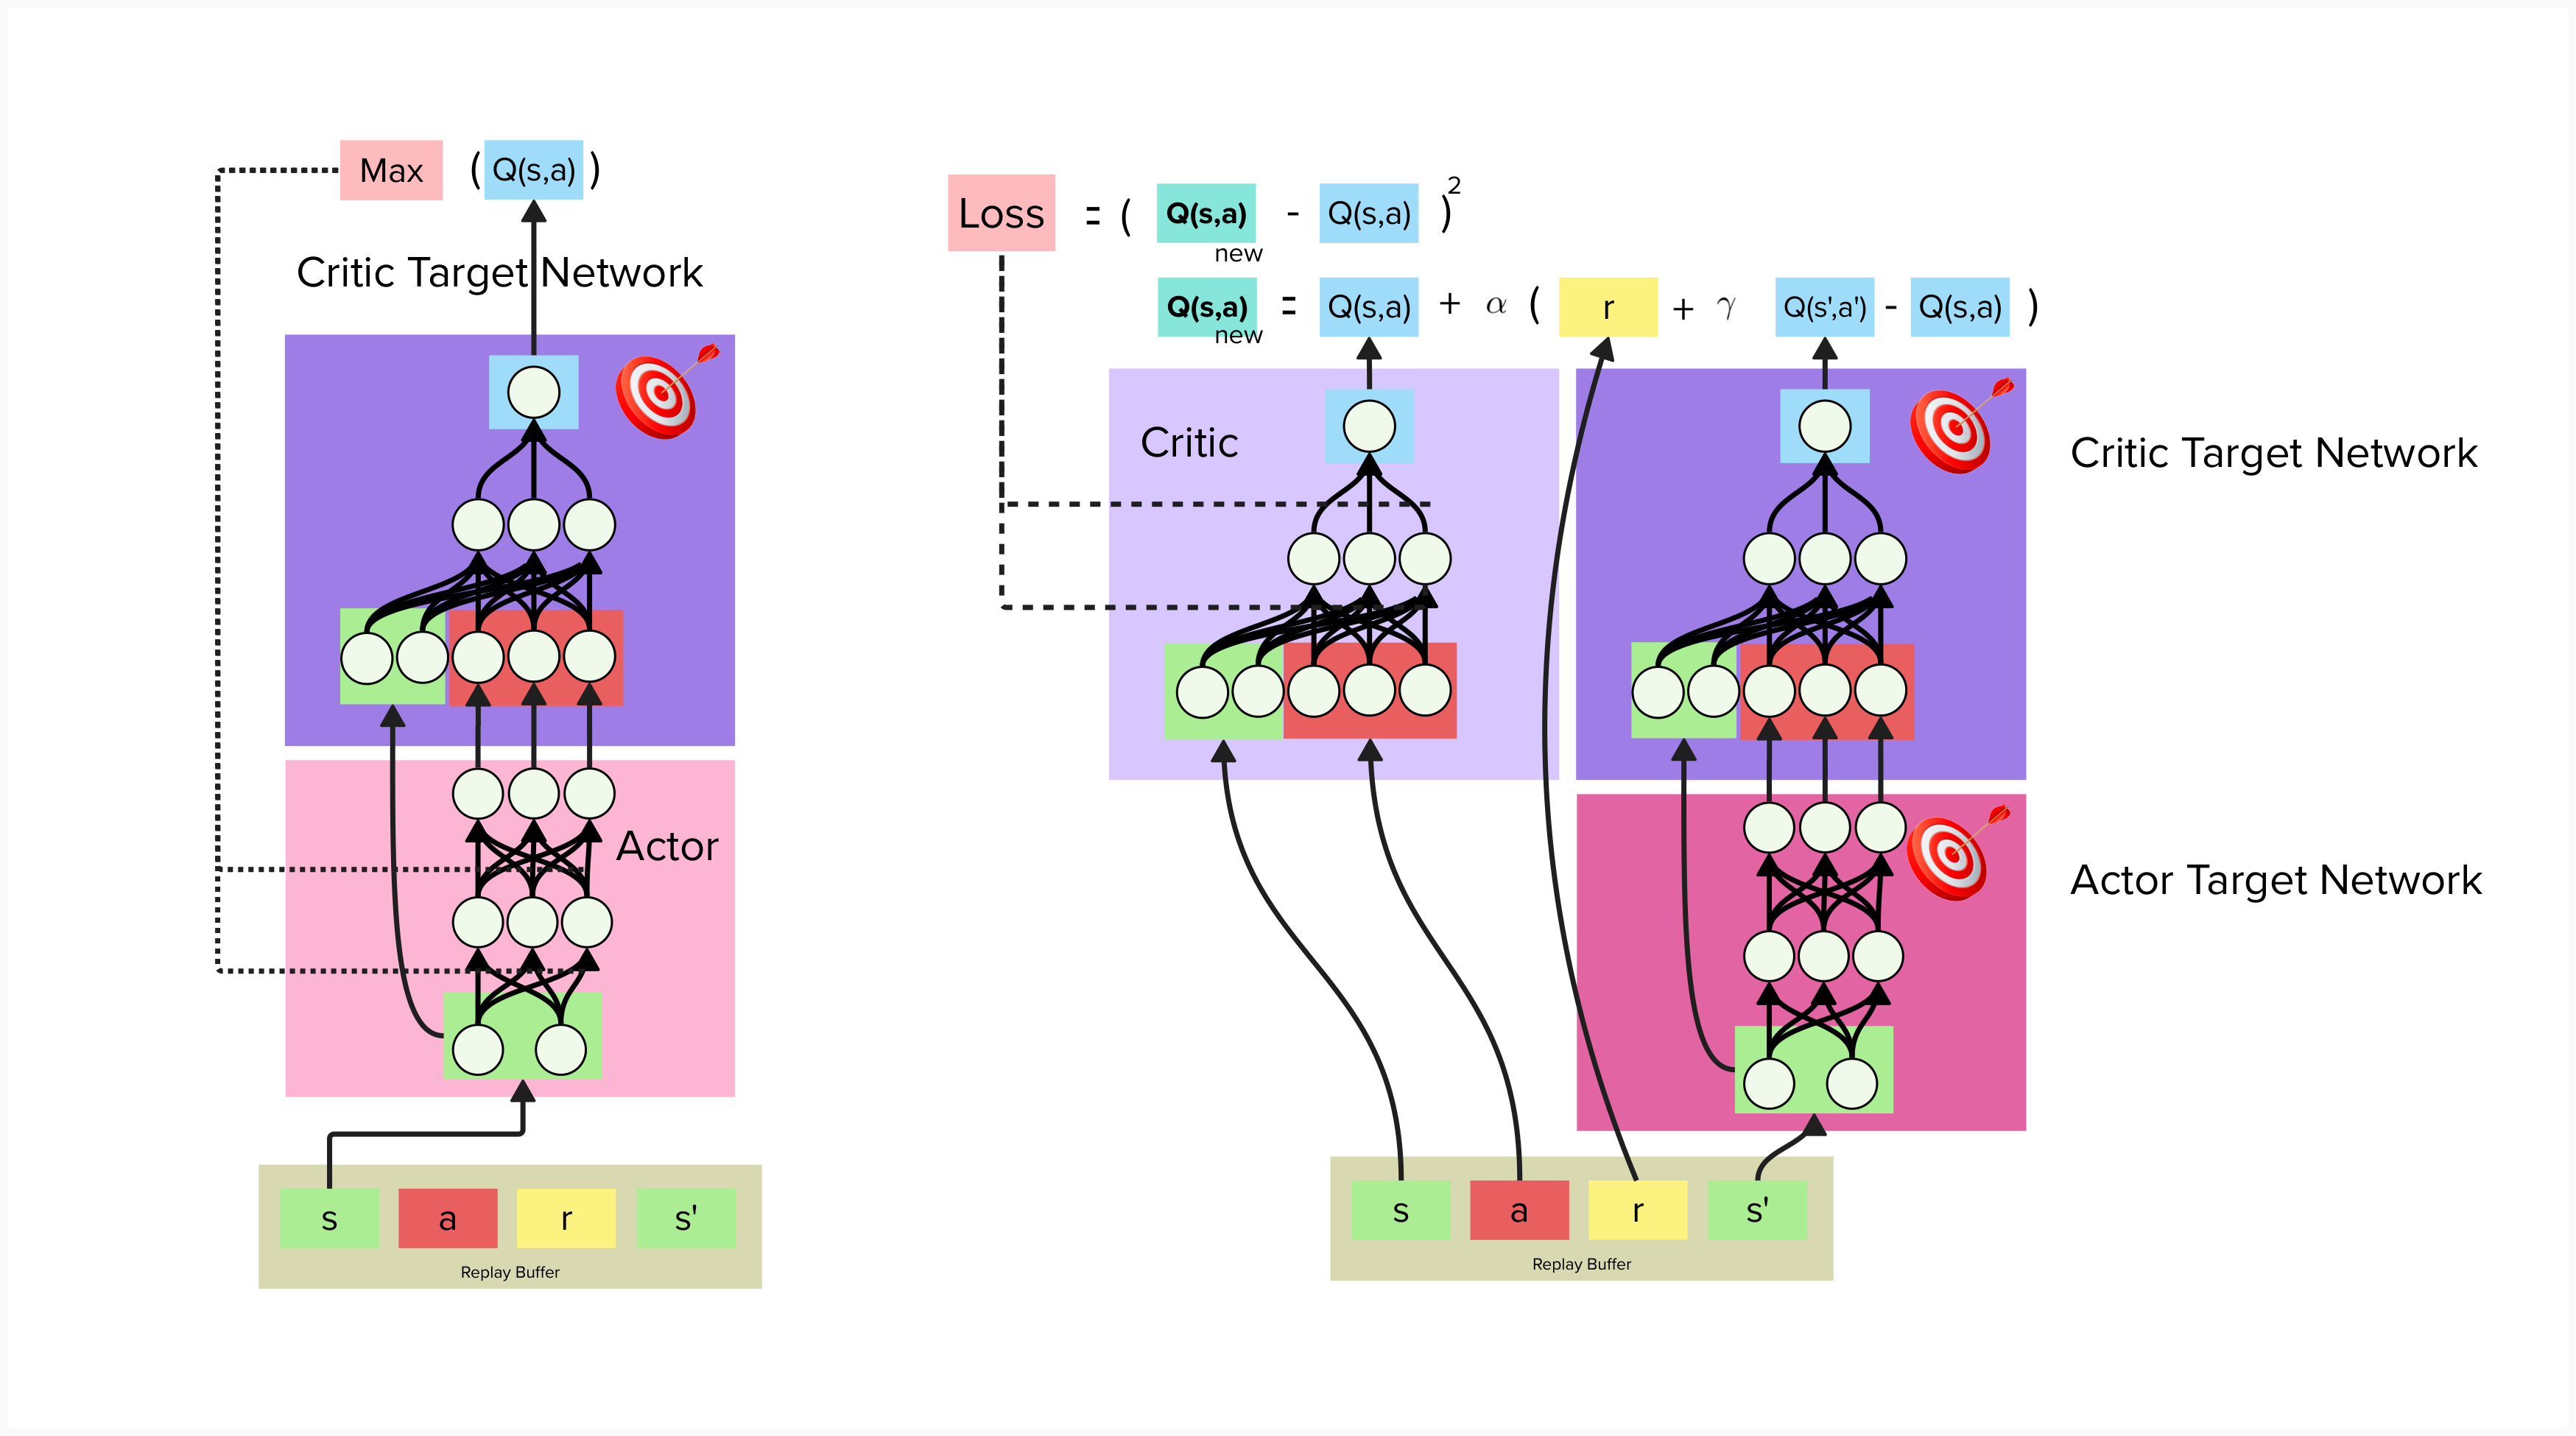
\includegraphics[width=0.99\textwidth, trim=10px 10px 10px 10px, clip]{2Grundlagen/35critick_actor_target.png}
\caption{Interaktion zwischen Actor, Critic und den Target Networks im DDPG-Algorithmus.}
\label{fig:actor_critic_diagram}
\end{figure}

\paragraph{Die Rolle der Target Networks im DDPG}
Im DDPG-Algorithmus werden Target Networks eingesetzt, um die Stabilität während des Trainings zu erhöhen. Diese Netzwerke sind Kopien des Critic und des Actor, die mit einem geringeren Update-Faktor \( \tau \) aktualisiert werden. Durch diese verzögerte Aktualisierung dienen die Target Networks als langsam veränderliche Zielwerte für die Updates des Critic und des Actor. Dies trägt dazu bei, die Korrelation zwischen den Schätzungen von \( Q(s,a) \) und \( Q(s',a') \) zu verringern und verhindert damit, dass der Lernalgorithmus durch schnelle Änderungen der bewerteten Policies instabil wird \cite{Wu2018AggregatedMultiDDPG}. Während des Trainingsprozesses bleibt das Target Network fest, das heißt, seine Gewichte werden nicht bei jedem Schritt aktualisiert, sondern in regelmäßigen Abständen, um die Stabilität der Zielwerte zu gewährleisten. Dies bedeutet, dass das Target Network als Ankerpunkt für den Actor und den Critic fungiert und ihnen eine konsistente Richtung für die Aktualisierung gibt. Insbesondere beim Update des Critics wird der TD-Fehler gegen die stabilen Zielwerte des Target Networks berechnet, was die Varianz der Updates reduziert und die Konvergenz des Netzwerks fördert. Beim Aktualisieren des Actors hingegen wird die Policy basierend auf einer Rückkopplung optimiert, die von den stabilen Q-Werten des Critic Target Networks abgeleitet ist. Die Verwendung von Target Networks im DDPG ist analog zum Einsatz des Experience Replay: Beide Techniken zielen darauf ab, die Korrelationen zwischen aufeinanderfolgenden Lernschritten zu reduzieren und die Datenvarianz zu erhöhen. Sie helfen dabei, eine stabilere und effektivere Lernumgebung zu schaffen, wie in der Forschung von \cite{Luck2019ImprovedExploration} und \cite{Wu2018AggregatedMultiDDPG} beschrieben.
 

\paragraph{Überleitung zu praktischen Anwendungen}
Nachdem die Grundlagenkapitel die Schlüsseltechniken des maschinellen Lernens, wie die Vorwärts- und Rückwärtspropagation, die Berechnung von Gradienten sowie verschiedene Netzwerkarchitekturen, eingeführt haben, steht nun die Anwendung dieser Methoden auf reale Probleme im Fokus. Im nächsten Kapitel werden wir die Leistungsfähigkeit von RL-Techniken an einem praktischen Beispiel demonstrieren: der Optimierung von PID-Reglern für die Steuerung von DC-DC-Wandlern. Unser Ziel ist es, einen Actor zu trainieren, der in der Lage ist, die PID-Koeffizienten präzise anzupassen, um auf verschiedene Degradationsstufen des Wandlers zu reagieren und somit seine Effizienz signifikant zu steigern. Diese Anwendung repräsentiert eine Brücke zwischen theoretischen Konzepten und realen ingenieurtechnischen Herausforderungen und zeigt, wie fortgeschrittene Algorithmen des maschinellen Lernens zur Lösung komplexer Steuerungsprobleme beitragen können.


